\begin{verbatim}
      . set graph on

      . //ON
\end{verbatim}

\subsection{Estadísticas de familia}\subsubsection{Proporción de casados y edad promedio de la esposa del asegurado titular}

En esta sección se clasifica al asegurado titular del IPS bajo las
siguientes condiciones:

\begin{itemize}
\item si tiene Seguro de Salud del IPS donde es el titular o,
\item si es cotizante al IPS o,
\item si cobra una jubilación y tiene seguro de IPS como jubilado o familiar del jubilado.
\end{itemize}

Por otra parte, es hijo/a dependiente de un asegurado titular del IPS si
tiene menos de 18 años de edad.

Un dato importante a la hora de realizar las proyecciones es la
proporción de casados, de manera a estimar la cantidad de potenciales
pensionados. En ese sentido, el 84\% de los jubilados de entre 60 y 69
años de edad están casados, poseen en promedio 2 (1,74) hijos y la edad
promedio de la esposa es de 66 años.

\begin{table}[H]
\begin{center}
\scriptsize
\caption{\bf{Características de la familia del trabajador asegurado titular del IPS}}
\begin{tabular}{l|rrrrrrrrrrrrrr}
\begin{tabular}{llllllllll}
\cline{1-10}
\multicolumn{1}{c}{} &
  \multicolumn{9}{|c}{Edad quinquenal} \\
\multicolumn{1}{c}{} &
  \multicolumn{1}{|r}{10 a 19} &
  \multicolumn{1}{r}{20 a 29} &
  \multicolumn{1}{r}{30 a 39} &
  \multicolumn{1}{r}{40 a 49} &
  \multicolumn{1}{r}{50 a 59} &
  \multicolumn{1}{r}{60 a 69} &
  \multicolumn{1}{r}{70 a 79} &
  \multicolumn{1}{r}{80 y más} &
  \multicolumn{1}{r}{Total} \\
\cline{1-10}
\multicolumn{1}{l}{Sexo} &
  \multicolumn{1}{|r}{} &
  \multicolumn{1}{r}{} &
  \multicolumn{1}{r}{} &
  \multicolumn{1}{r}{} &
  \multicolumn{1}{r}{} &
  \multicolumn{1}{r}{} &
  \multicolumn{1}{r}{} &
  \multicolumn{1}{r}{} &
  \multicolumn{1}{r}{} \\
\multicolumn{1}{l}{\hspace{1em}Hombres} &
  \multicolumn{1}{|r}{} &
  \multicolumn{1}{r}{} &
  \multicolumn{1}{r}{} &
  \multicolumn{1}{r}{} &
  \multicolumn{1}{r}{} &
  \multicolumn{1}{r}{} &
  \multicolumn{1}{r}{} &
  \multicolumn{1}{r}{} &
  \multicolumn{1}{r}{} \\
\multicolumn{1}{l}{\hspace{2em}Proporción de Casados/as} &
  \multicolumn{1}{|r}{.} &
  \multicolumn{1}{r}{0,44} &
  \multicolumn{1}{r}{0,81} &
  \multicolumn{1}{r}{0,87} &
  \multicolumn{1}{r}{0,88} &
  \multicolumn{1}{r}{0,84} &
  \multicolumn{1}{r}{0,85} &
  \multicolumn{1}{r}{0,59} &
  \multicolumn{1}{r}{0,88} \\
\multicolumn{1}{l}{\hspace{2em}Edad promedio de la esposa/o} &
  \multicolumn{1}{|r}{.} &
  \multicolumn{1}{r}{21,81} &
  \multicolumn{1}{r}{29,74} &
  \multicolumn{1}{r}{38,07} &
  \multicolumn{1}{r}{47,24} &
  \multicolumn{1}{r}{55,80} &
  \multicolumn{1}{r}{66,69} &
  \multicolumn{1}{r}{72,83} &
  \multicolumn{1}{r}{72,83} \\
\multicolumn{1}{l}{\hspace{2em}Nro promedio de hijos/as} &
  \multicolumn{1}{|r}{1,62} &
  \multicolumn{1}{r}{1,61} &
  \multicolumn{1}{r}{1,93} &
  \multicolumn{1}{r}{2,42} &
  \multicolumn{1}{r}{2,37} &
  \multicolumn{1}{r}{1,74} &
  \multicolumn{1}{r}{.} &
  \multicolumn{1}{r}{.} &
  \multicolumn{1}{r}{2,42} \\
\multicolumn{1}{l}{\hspace{2em}Edad promedio del hijo/a} &
  \multicolumn{1}{|r}{3,52} &
  \multicolumn{1}{r}{3,83} &
  \multicolumn{1}{r}{6,45} &
  \multicolumn{1}{r}{10,32} &
  \multicolumn{1}{r}{11,43} &
  \multicolumn{1}{r}{11,43} &
  \multicolumn{1}{r}{.} &
  \multicolumn{1}{r}{.} &
  \multicolumn{1}{r}{11,43} \\
\multicolumn{1}{l}{\hspace{1em}Mujeres} &
  \multicolumn{1}{|r}{} &
  \multicolumn{1}{r}{} &
  \multicolumn{1}{r}{} &
  \multicolumn{1}{r}{} &
  \multicolumn{1}{r}{} &
  \multicolumn{1}{r}{} &
  \multicolumn{1}{r}{} &
  \multicolumn{1}{r}{} &
  \multicolumn{1}{r}{} \\
\multicolumn{1}{l}{\hspace{2em}Proporción de Casados/as} &
  \multicolumn{1}{|r}{.} &
  \multicolumn{1}{r}{0,39} &
  \multicolumn{1}{r}{0,68} &
  \multicolumn{1}{r}{0,70} &
  \multicolumn{1}{r}{0,68} &
  \multicolumn{1}{r}{0,62} &
  \multicolumn{1}{r}{0,48} &
  \multicolumn{1}{r}{0,25} &
  \multicolumn{1}{r}{0,70} \\
\multicolumn{1}{l}{\hspace{2em}Edad promedio de la esposa/o} &
  \multicolumn{1}{|r}{.} &
  \multicolumn{1}{r}{25,88} &
  \multicolumn{1}{r}{34,12} &
  \multicolumn{1}{r}{43,94} &
  \multicolumn{1}{r}{53,86} &
  \multicolumn{1}{r}{65,71} &
  \multicolumn{1}{r}{71,56} &
  \multicolumn{1}{r}{81,44} &
  \multicolumn{1}{r}{81,44} \\
\multicolumn{1}{l}{\hspace{2em}Nro promedio de hijos/as} &
  \multicolumn{1}{|r}{.} &
  \multicolumn{1}{r}{1,50} &
  \multicolumn{1}{r}{1,99} &
  \multicolumn{1}{r}{2,31} &
  \multicolumn{1}{r}{1,63} &
  \multicolumn{1}{r}{.} &
  \multicolumn{1}{r}{.} &
  \multicolumn{1}{r}{.} &
  \multicolumn{1}{r}{2,31} \\
\multicolumn{1}{l}{\hspace{2em}Edad promedio del hijo/a} &
  \multicolumn{1}{|r}{.} &
  \multicolumn{1}{r}{4,00} &
  \multicolumn{1}{r}{7,34} &
  \multicolumn{1}{r}{11,42} &
  \multicolumn{1}{r}{13,25} &
  \multicolumn{1}{r}{.} &
  \multicolumn{1}{r}{.} &
  \multicolumn{1}{r}{.} &
  \multicolumn{1}{r}{13,25} \\
\multicolumn{1}{l}{\hspace{1em}Total} &
  \multicolumn{1}{|r}{} &
  \multicolumn{1}{r}{} &
  \multicolumn{1}{r}{} &
  \multicolumn{1}{r}{} &
  \multicolumn{1}{r}{} &
  \multicolumn{1}{r}{} &
  \multicolumn{1}{r}{} &
  \multicolumn{1}{r}{} &
  \multicolumn{1}{r}{} \\
\multicolumn{1}{l}{\hspace{2em}Proporción de Casados/as} &
  \multicolumn{1}{|r}{.} &
  \multicolumn{1}{r}{0,44} &
  \multicolumn{1}{r}{0,81} &
  \multicolumn{1}{r}{0,87} &
  \multicolumn{1}{r}{0,88} &
  \multicolumn{1}{r}{0,84} &
  \multicolumn{1}{r}{0,85} &
  \multicolumn{1}{r}{0,59} &
  \multicolumn{1}{r}{0,88} \\
\multicolumn{1}{l}{\hspace{2em}Edad promedio de la esposa/o} &
  \multicolumn{1}{|r}{.} &
  \multicolumn{1}{r}{25,88} &
  \multicolumn{1}{r}{34,12} &
  \multicolumn{1}{r}{43,94} &
  \multicolumn{1}{r}{53,86} &
  \multicolumn{1}{r}{65,71} &
  \multicolumn{1}{r}{71,56} &
  \multicolumn{1}{r}{81,44} &
  \multicolumn{1}{r}{81,44} \\
\multicolumn{1}{l}{\hspace{2em}Nro promedio de hijos/as} &
  \multicolumn{1}{|r}{1,62} &
  \multicolumn{1}{r}{1,61} &
  \multicolumn{1}{r}{1,99} &
  \multicolumn{1}{r}{2,42} &
  \multicolumn{1}{r}{2,37} &
  \multicolumn{1}{r}{1,74} &
  \multicolumn{1}{r}{.} &
  \multicolumn{1}{r}{.} &
  \multicolumn{1}{r}{2,42} \\
\multicolumn{1}{l}{\hspace{2em}Edad promedio del hijo/a} &
  \multicolumn{1}{|r}{3,52} &
  \multicolumn{1}{r}{4,00} &
  \multicolumn{1}{r}{7,34} &
  \multicolumn{1}{r}{11,42} &
  \multicolumn{1}{r}{13,25} &
  \multicolumn{1}{r}{11,43} &
  \multicolumn{1}{r}{.} &
  \multicolumn{1}{r}{.} &
  \multicolumn{1}{r}{13,25} \\
\cline{1-10}
\end{tabular}

\end{tabular}
                                    \item \footnotesize Fuente : Encuesta Permanente de Hogares.
                    %\item \footnotesize Nota : Trabajadores ocupados mayores de 14 años.
\end{center}
\end{table}

\begin{figure}[H]
\begin{center}
                    \caption{Proporción de casados por edad y sexo del asegurado titular}
                    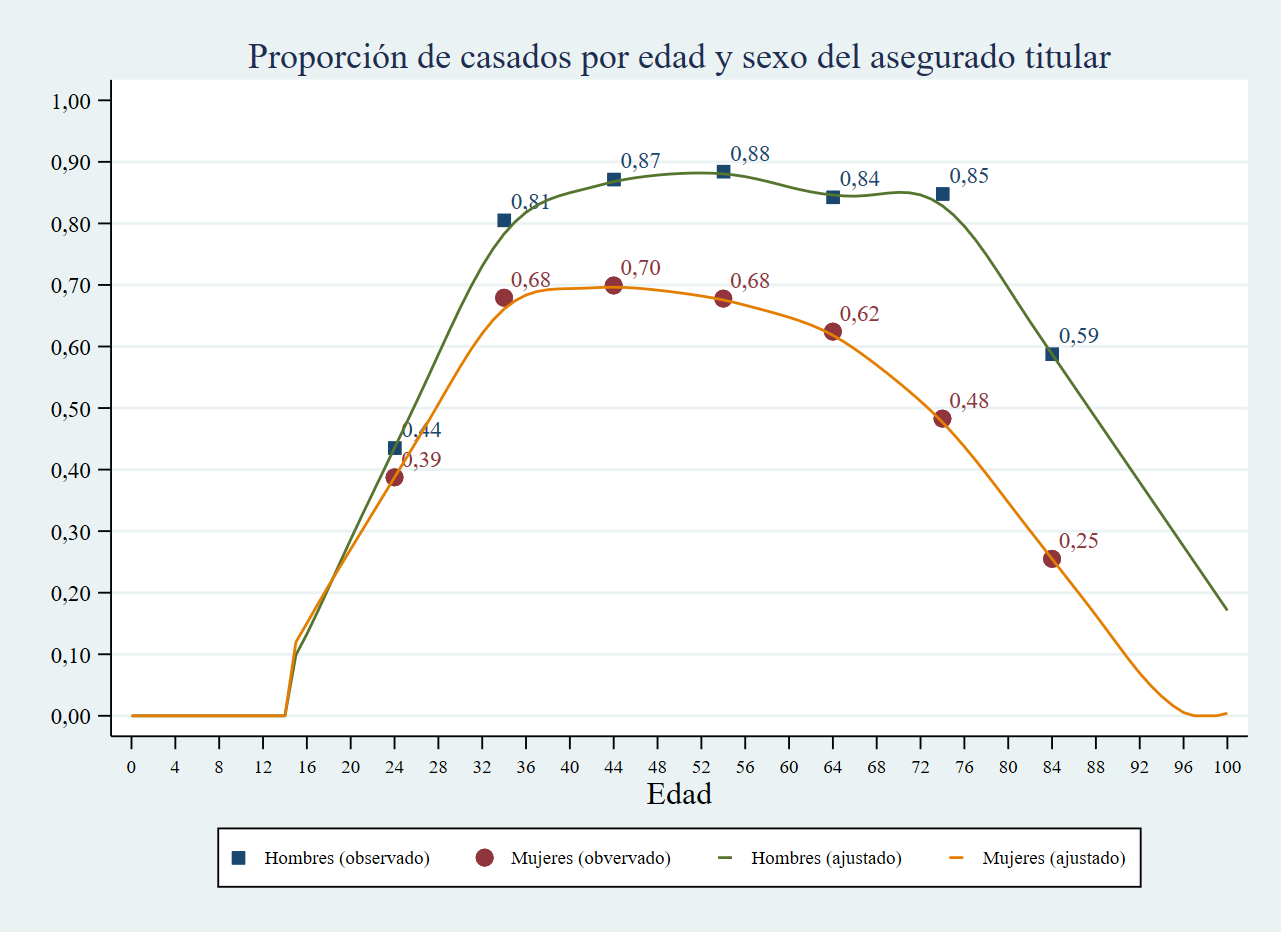
\includegraphics[scale=0.35]{EPH_familia_prop_casado.png}
                                    \item \footnotesize Fuente : Encuesta Permanente de Hogares.
                                    \item \footnotesize Nota : 
                    \end{center}
\end{figure}

\begin{figure}[H]
\begin{center}
                    \caption{Edad promedio de la esposa y del esposo por edad y sexo del asegurado titular}
                    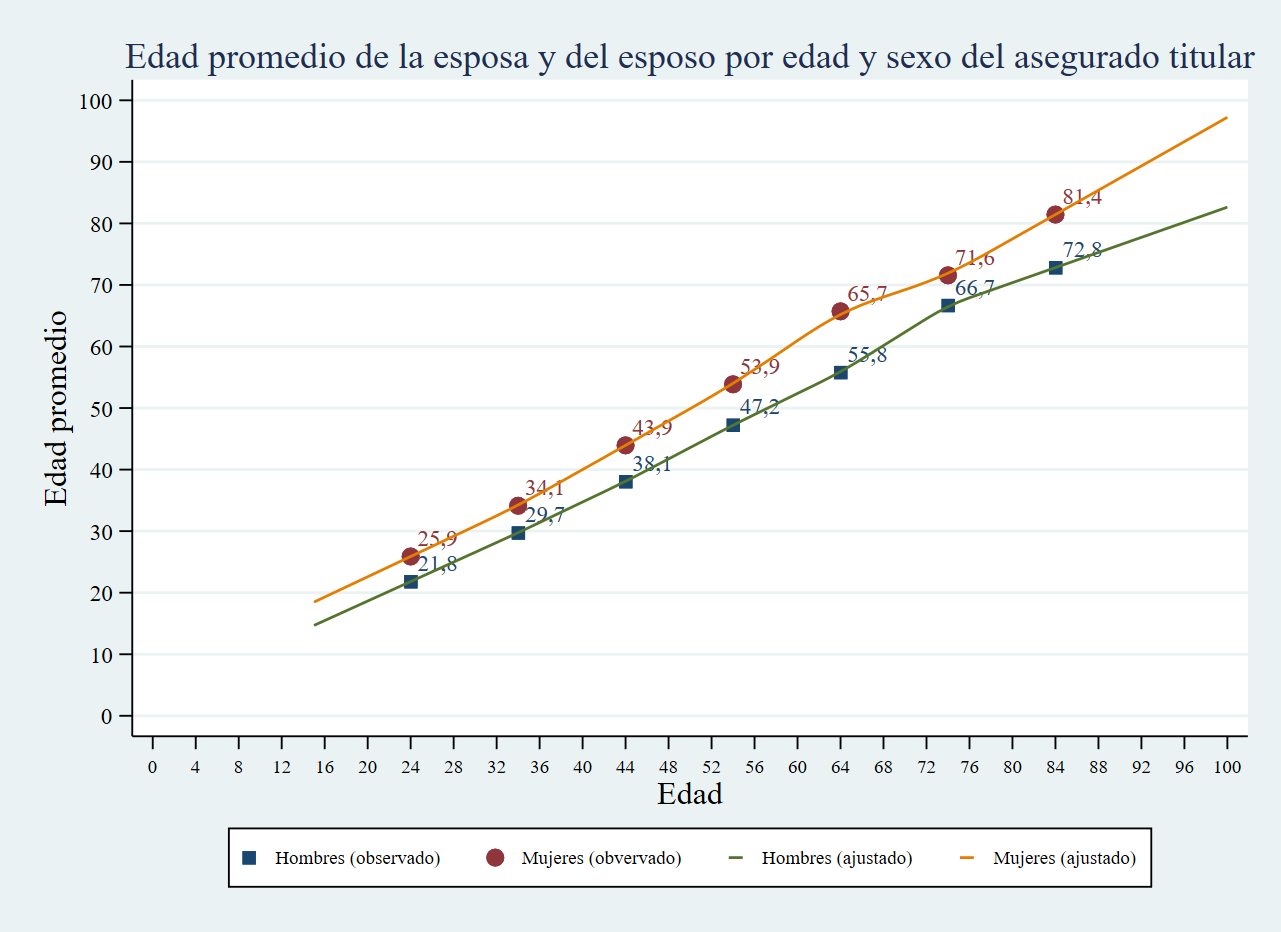
\includegraphics[scale=0.35]{EPH_familia_edadmed_esposa.png}
                                    \item \footnotesize Fuente : Encuesta Permanente de Hogares.
                                    \item \footnotesize Nota : 
                    \end{center}
\end{figure}

\subsubsection{Cantidad promedio y edad promedio de los hijos del asegurado titular}

Es hijo/a dependiente de un asegurado titular del IPS si tiene menos de
18 años de edad.

\begin{figure}[H]
\begin{center}
                    \caption{Cantidad promedio de hijos dependientes por edad y sexo del asegurado titular}
                    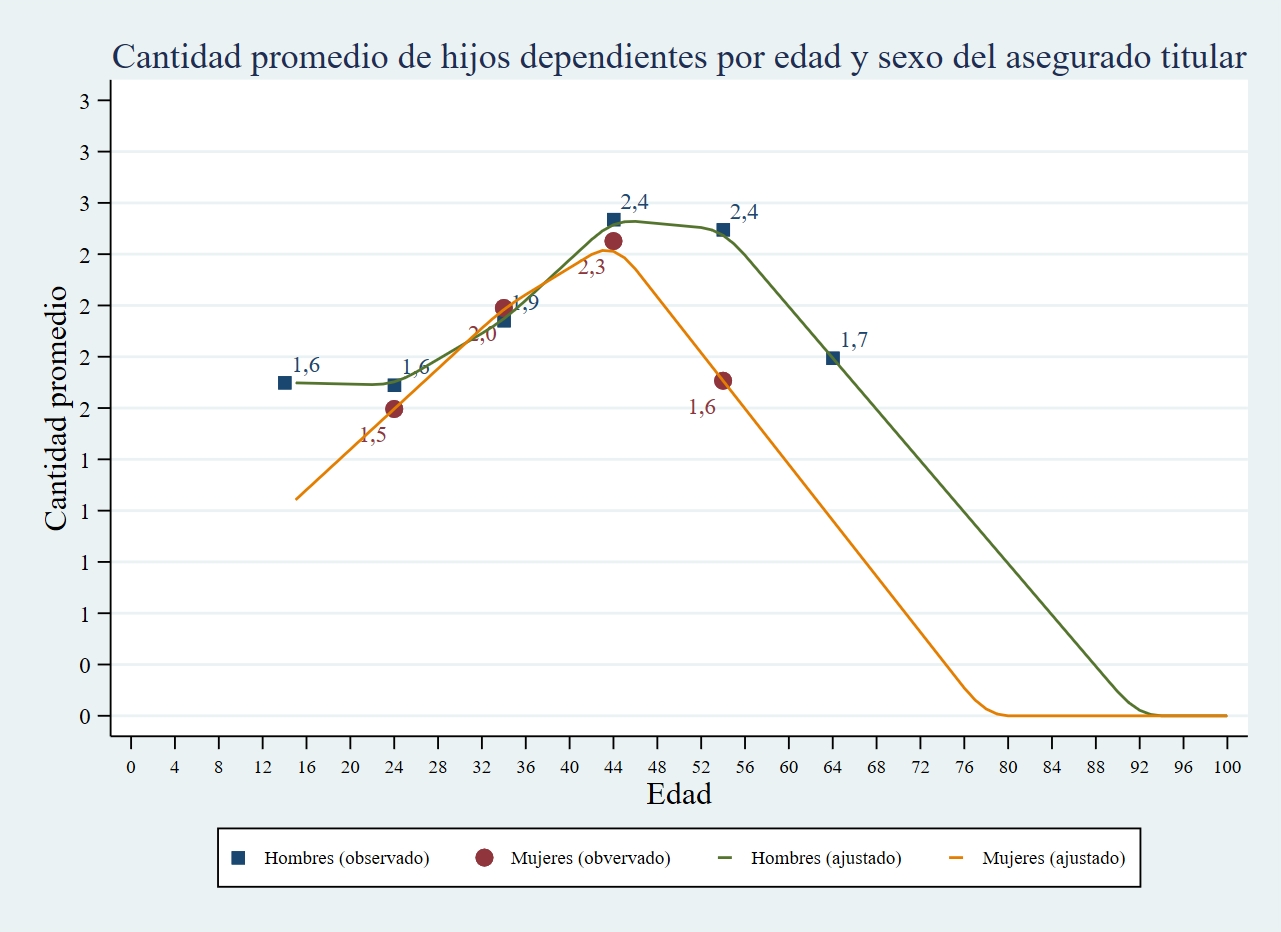
\includegraphics[scale=0.35]{EPH_familia_nro_prom_hijos.png}
                                    \item \footnotesize Fuente : Encuesta Permanente de Hogares.
                                    \item \footnotesize Nota : 
                    \end{center}
\end{figure}

\begin{figure}[H]
\begin{center}
                    \caption{Edad promedio de los hijos dependientes por edad y sexo del asegurado titular}
                    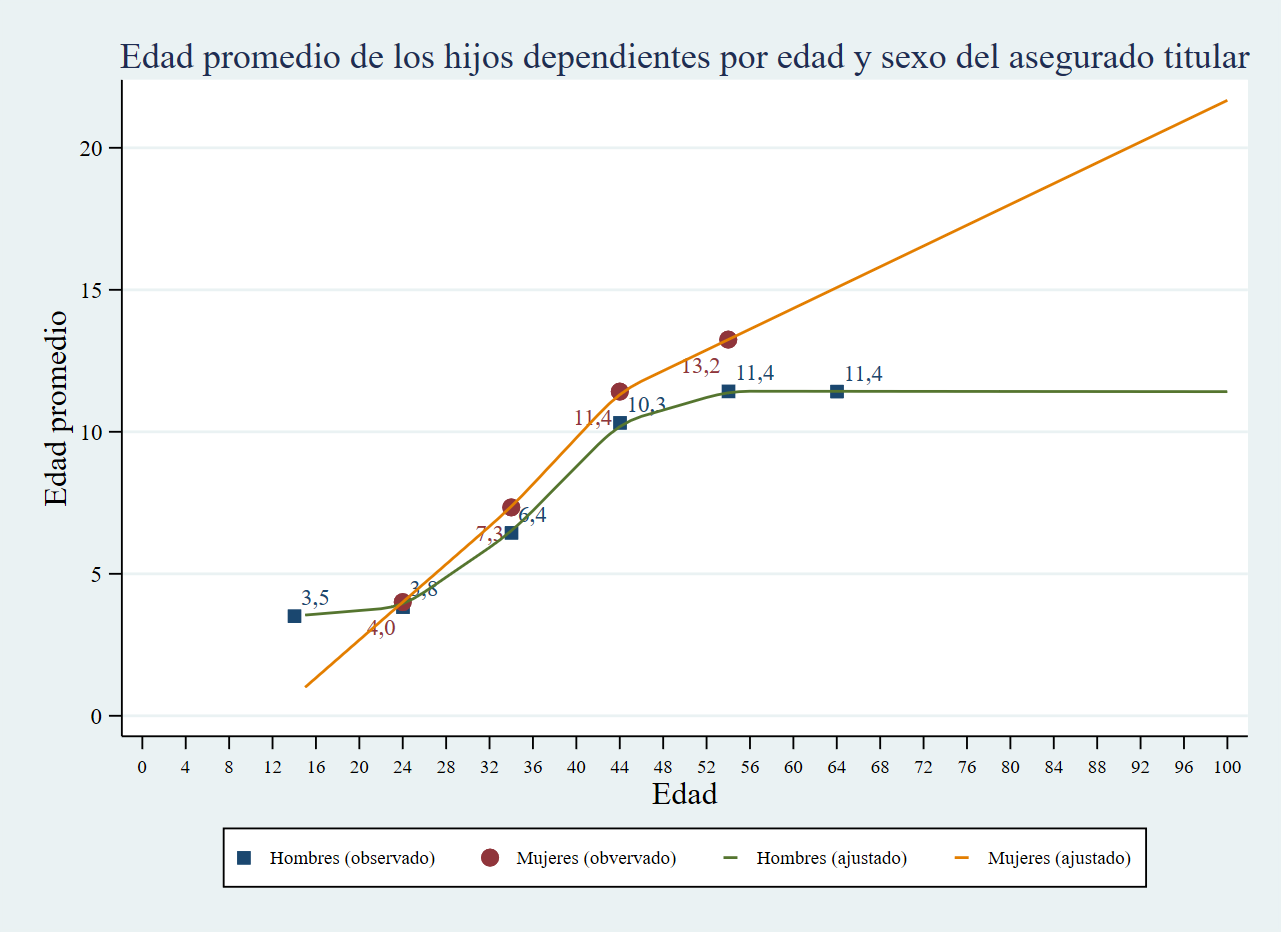
\includegraphics[scale=0.35]{EPH_familia_edad_prom_hijos.png}
                                    \item \footnotesize Fuente : Encuesta Permanente de Hogares.
                                    \item \footnotesize Nota : 
                    \end{center}
\end{figure}
